 \section{Predictability, Complexity, and Permutation Entropy} % (fold)
 \label{sec:results}
% I changed the title of this section because there are lots of
% results in the modeling section too.  The results HERE are about the
% relationship between predictability and WPE


%OUTLINE:
%\begin{enumerate}
%\item \cmark~Introduce MASE.
%\item \cmark~WPE is a good measure of predictability.  %Figure: best athlete MASE vs.
%its WPE.
%\item \cmark~Talk about structure analysis. Just because %there is forward information
%transfer, does not mean that linear predictors can get at %this.
%\subitem \cmark~For this show a figure of (a) ARIMA vs MASE %(b) LMA vs MASE in a side by%
%side plot.
%\item full results.  Image: MASE vs. WPE for both LMA \& %ARIMA.  Points to make:
%\begin{enumerate}
%\item \cmark~clusters are distributed differently
%\item \cmark~clusters are shaped differently---tight or not
%\item \cmark~clusters move differently between LMA and ARIMA
%\item finally, the diagonal line is important. If you're %below it, you could do
%better.
%\end{enumerate}
%\end{enumerate}

%BRAINSTORMING 
%\begin{itemize}
%\cmark\item The kind of complexity present matters, i.e., that is whether the complexity is structured or not.[[use here and mention in intro]] 
%\cmark\item Quantifying structured and unstructured complexity is nontrivial in the case of real-valued noisy time series but WPE does this. [[talk about again here but justify in information theory section]]
%\item Maybe plot a big chunk of \col and a big chunk of \gcc together and show that they both look complex. 

%\cmark\item \gcc appears visually very complex, *and* according to WPE this complexity is unstructured. And a constant, linear and nonlinear prediction strategy all fail. We should be able to conclude that guessing random values is the best we can do as is shown by MASE [[Use in this section]]

%\cmark\item \col is also complex (can even be chaotic/ point to CHAOS paper) but the complexity is structured according to WPE and as such that complexity is usable for prediction [[use in this section]]

%\cmark\item \col brings about the point nicely that some prediction strategies cannot utilize the processes internal information transfer method. That is a nonlinear internal information transfer system cannot be predicted effectively with a linear strategy. This gives a practitioner leverage on when to give up and when to keep working. [[use in this section as bridge to next section]]

%\end{itemize}

In this section, we offer an empirical validation of the two key
conjectures introduced in Section \ref{sec:intro}, namely:

\begin{enumerate}

\item that the weighted permutation entropy (WPE) of a noisy
  real-valued time series is correlated with prediction
  accuracy---i.e., that the predictable structure in a time-series
  data set can be quantified by its WPE.

%\subitem [[Simply reminders not to be included]]WPE can quantify when
%a noisy real-valued time series is predictable.[[I am unsatisfied
%with predictable in this sentence, need a better word to say "better
%than random walk" or ``able to be forecast effectively" or ``has the
%structural capacity to transmit information in a way that the time
%series can be effectively forecast"

%\item The existence of complex structure in a noisy real-valued time
%series is quantifiable and this type of complexity is directly
%correlated with predictability

\item that the way information is processed internally by a system is
  correlated with the effectiveness of a given predictor on
  time-series data from that system

%\subitem [[Simply reminders not to be included]]We will have shown
%that the existence whether linear or nonlinear is picked up on with
%WPE but this point gets at whether the prediction model can use the
%structure or not (linear can't use nonlinear structure). The right to
%left shifts in \col and some of the \svd regimes and the lack of
%shift in \gcc illustrate this nicely.

%\subitem [[Simply reminders not to be included]]This is the linear vs
%nonliear vs random we see with the right to left shifts with lower
%complexity time series.

\end{enumerate}

%This portion should justify the following claim%%%%%%%%%%%%%%%%%%%%%%
%\item The existence of predictable structure in noisy real-valued time series is quantifiable by WPE and as a result WPE is correlated with prediction accuracy (MASE)  
%%%%%%%%%%%%%%%%%%%%%%%%%





%\item First paragraph: WPE is a good measure of predictability.  Figure:
%best athlete MASE vs. its WPE. 


%\item Quantifying structured and unstructured complexity is
%nontrivial in the case of real-valued noisy time series but WPE does
%this. [[talk about again here but justify in information theory
%section]]

The experiments below involve the three different prediction methods
described in Section~\ref{sec:compModel}---na\"ive, ARIMA, and
LMA---applied to time-series data from eight different systems: {\tt
  col\_major}, {\tt 403.gcc}, and the six different regimes of the
{\tt dgesdd} signal in Figure~\ref{fig:wwpe}.  The objective of these
experiments was to explore how prediction accuracy is related to WPE,
and how that relationship depends on the generating process and the
prediction method.  Working from the first 90\% of each signal, we
generated a prediction of the last 10\% of that signal using each of
the methods, as described in Section~\ref{sec:accuracy}, then
calculated the MASE value of those predictions.  We also calculated
the WPE of each time series, as described in
Section~\ref{sec:meaComplex}, using a wordlength of six.  In order to
assess the run-to-run variability of these results, we repeated all of
these calculations on 15 separate trials: i.e., 15 different runs of
each program.  Figure~\ref{fig:wpe_vs_mase_best} shows the {\sl best}
of these 45 predictions for each system: i.e., the lowest error over
all 15 trials and all three methods for each program.  The WPE is
plotted against the corresponding MASE value in order to bring out the
correlation between these two quantities.
\begin{figure}[htbp]
  \centering
  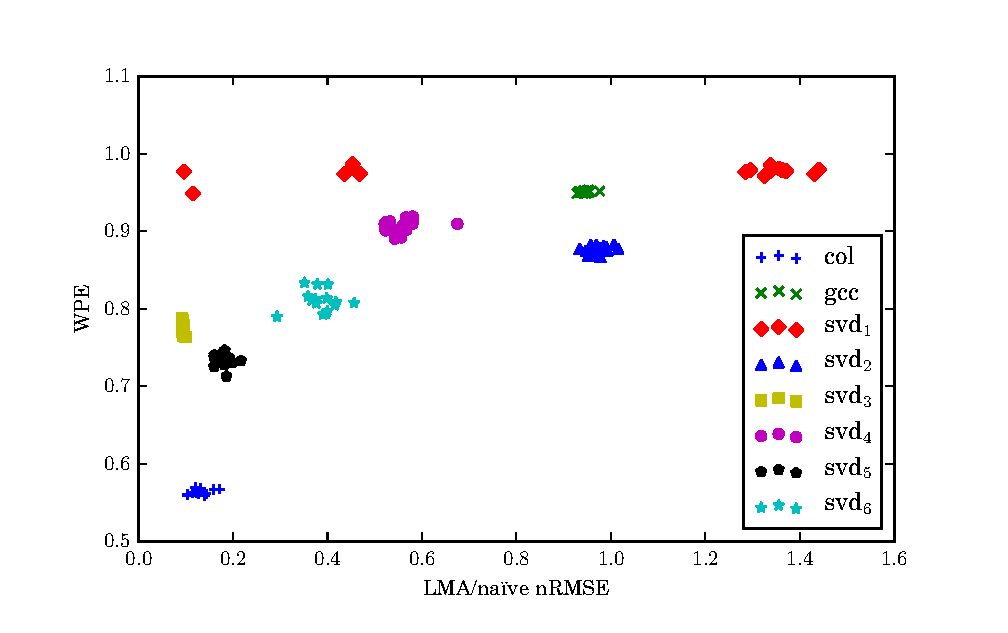
\includegraphics[width=0.6\textwidth]{figs/prediction_vs_entropy}
  \caption{Weighted permutation entropy vs. mean absolute scaled error
    (MASE) of the best prediction of each system.
% 
% (across all trials and all prediction methods) 
% 
The dashed line is a least-squares linear fit of all the points except
{\tt dgesdd$_1$}, which we have excluded for reasons explained in the
text.  [[Ryan, is that correct?]]}
  \label{fig:wpe_vs_mase_best}
\end{figure}

The best-case prediction error for each of these eight systems is
roughly proportional to the weighted permutation entropy, which is
consistent with our first conjecture.  The dashed line in the figure,
a linear least-squares fit to these best-case errors---with the
exception of {\tt dgesdd$_5$}, for reasons described below---captures
this rough proportionality.  This is not a formal result.  The three
methods used here were chosen to span the space of standard prediction
strategies, but they do not, of course, cover that space exhaustively.
Our goal here is an empirical assessment of predictability and
complexity, not formal results about a ``best'' predictor for a given
time series.  There may be other methods that produce lower MASE
values than those in Figure~\ref{fig:wpe_vs_mase_best}, but the
sparseness of the points in the upper-left and lower-right quadrants
of this plot strongly suggests that the underlying predictability of a
time series is inversely correlated with its WPE.  The rest of this
section describes our results in more detail, including the measures
taken to assure meaningful comparisons across methods, trials, and
programs, and elaborates on the meaning of the dashed line in the
figure.

Figure~\ref{fig:wpe_vs_mase_all} shows WPE vs. MASE plots for all 360
experiments.
\begin{figure}
  \centering
    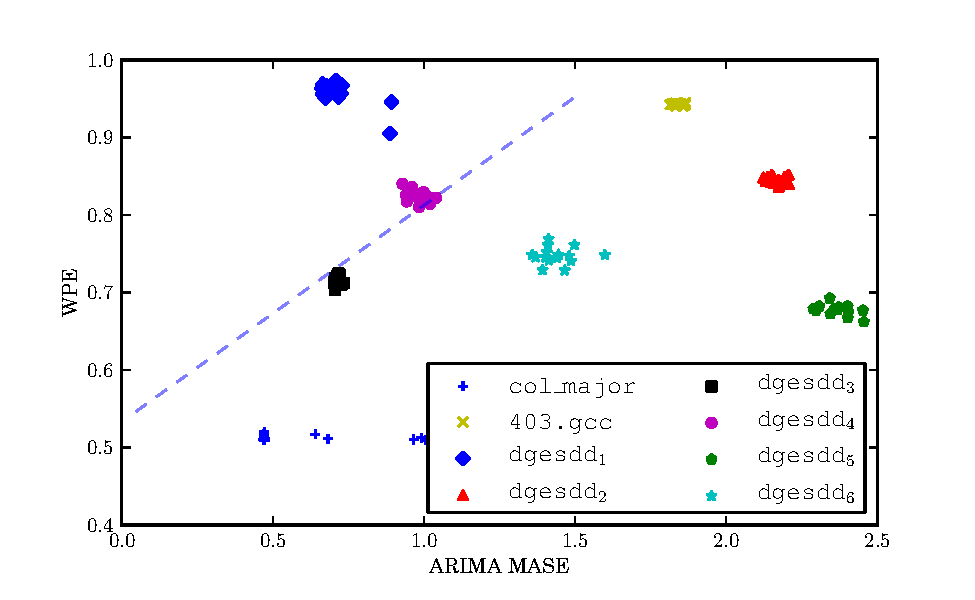
\includegraphics[width=0.6\textwidth]{figs/ARIMA_prediction_vs_entropy}
    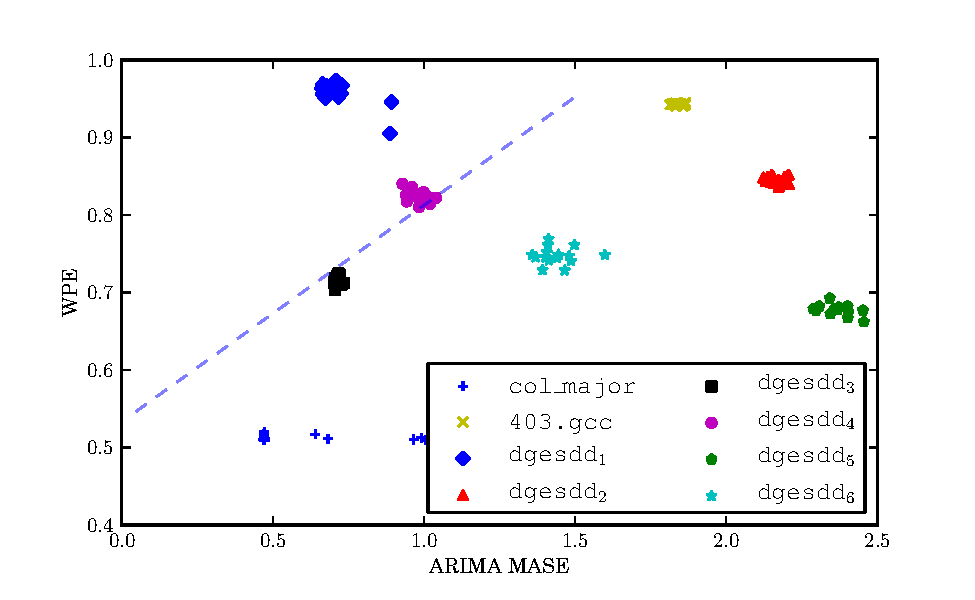
\includegraphics[width=0.6\textwidth]{figs/ARIMA_prediction_vs_entropy}
    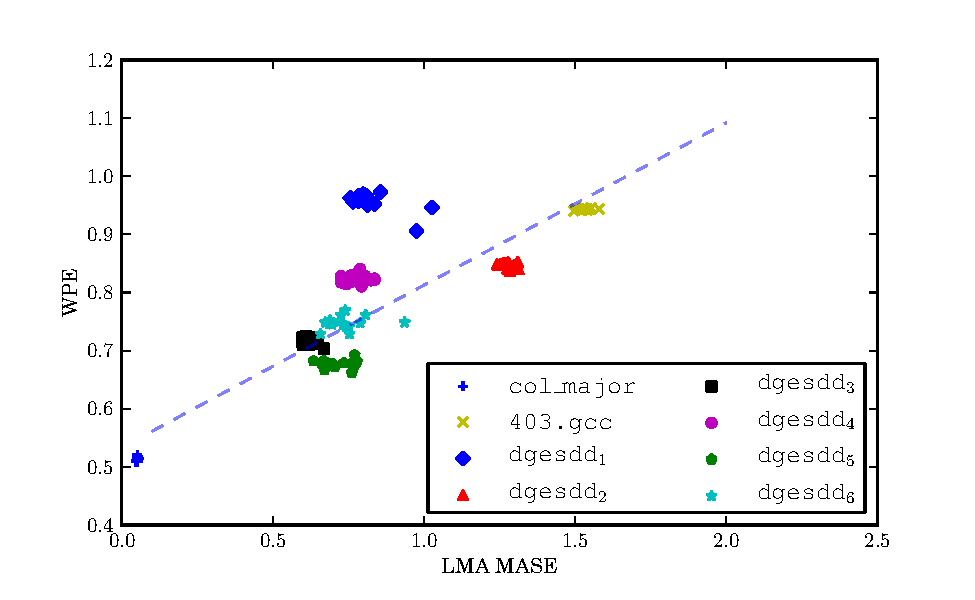
\includegraphics[width=0.6\textwidth]{figs/LMA_prediction_vs_entropy}
\caption{WPE vs. MASE for all trials, methods, and systems.  \svdone,
  \svdthree, and \svdfive are omitted from the top plot for scale
  reasons; their MASE scores are $2.6763\pm4.3282$, $31.3857\pm
  0.2820$, and $20.8703 \pm 0.1915$ respectively.  {\color{red}Replace
    the top plot with a plot of the naive results---but running from 0
    to 3.1 on the horizontal axis and excluding SVD 1, 3, and 5}.  The
  dashed line is the same as in the previous figure [[Ryan, is this
      correct?]].  Numerical values, including means and standard
  deviations of the errors, can be found in Table~\ref{tab:error} in
  the appendix.
% 
%  [[All traces except those from \svd$_1$ lie above the line,
%      indicating that LMA is better suited prediction method for the
%      computer traces considered.]]  [[This comes {\bf long} before the
%      associated discussion in the text, and it's not what this figure
%      is trying to show here.]]
% 
}
    \label{fig:wpe_vs_mase_all}
\end{figure} 
There are 15 points in each cluster, one for each trial\footnote{A
  trial involves collecting a time series from the corresponding
  system, predicting the last 10\% of that time series, and
  calculating the MASE score.}.  (The points in
Figure~\ref{fig:wpe_vs_mase_best} are the leftmost points in any of
the three clusters for the corresponding system.)  Most of the
clusters are quite tight.  Some are flat and wide because the WPE
values of each run of any particular program tend to have little
variance; for most traces, the LMA and ARIMA variance is low as well,
resulting in small, tight clusters.  The {\sl spatial distribution} of
the clusters is quite different in the three plots: LMA is tight
around the dashed line, whereas naive and ARIMA are [[need to fill in
    words here when get the third image]].  This is a geometric
validation of the second conjecture in this paper, as described in the
following paragraphs.

Though \col is a very simple program, its dynamics are actually quite
complicated, as discussed in Section~\ref{sec:intro}.  Recall from the
right-hand column of Figure~\ref{fig:gcc_vs_col} that the naive and
ARIMA prediction methods perform poorly on this signal (MASE values
$0.57 \pm$ 0.001 and $0.59 \pm 0.21$, respectively).  That is, the
errors produced by these methods are a little over half as large as
the errors produced by the random-walk method, which simply uses the
current value as the prediction.  However, the WPE value for the \col
trials is $0.51 \pm 0.003$: i.e., right in the middle of the
complexity spectrum described in Section~\ref{sec:intro}, implying
that roughly half of the signal is predictive structure.  This
disparity---WPE values that suggest a high rate of forward information
transfer in the signal, but predictions with low MASE
scores---manifests geometrically in the top two images in
Figure~\ref{fig:wpe_vs_mase_all}, where the \col clusters are far to
the right of the dashed line.  This is important; it says that the
methods aren't leveraging that information very well.  This is not
surprising, really.  The dynamics of \col may be complicated, but they
are not unstructured.  This signal is nonlinear, deterministic, and
chaotic.  Indeed, if you use a prediction technique that uses a
nonlinear model (LMA) you get a MASE of $0.05 \pm 0.001$---i.e., 20
times more accurate than a random-walk forecast.  Note the position of
the \col cluster in the bottom image in
Figure~\ref{fig:wpe_vs_mase_all}: much closer to the dashed line.
From a practitioner's standpoint, what this means is that being below
that line tells you that there really IS usable structure in the time
series, that you could do better, and that you should use a better
method.  Note, too, that the \col points are clustered in LMA but
spread out horizontally in ARIMA, far to the right of the dashed line
(i.e., much worse than the other methods).  We need to come up with a
hypothesis about this spread and skew, even if it's totally tentative.

The WPE of \svdfive ($0.677 \pm 0.006$) is higher than that of {\tt
  col\_major}.  This indicates that the rate of forward information
transfer of the underlying process is lower, but that time-series data
from this system still contain a significant amount of structure that
can, in theory, be leveraged to predict the future course of the time
series.  However, the effectiveness of any prediction strategy will
depend on how well it leverages the available information.
% 
% (This is the basis for the second conjecture above.)  
% 
This issue becomes apparent in the case of \svdfive, as is clear from
the positions of the corresponding clusters in
Figure~\ref{fig:wpe_vs_mase_all}.  The naive and ARIMA prediction
strategies in the top two plots produce MASE scores of $2.3700 \pm
0.0505 $ and $20.8703 \pm 0.1915$, respectively: that is, 2.37 and
20.87 times worse than a simple random walk forecast of the same
signals.  [[This is big because the amount of variance in this signal
    makes it a bad idea to just guess the mean.  The same thing is
    true of \svdthree.]] [[Joshua: can you say that better---in a way
    that is true of both of these, and distinguishes them from all of
    the signals that have lower values?]] Again, the positions of the
ARIMA and LMA clusters---significantly below and to the right of the
dashed line---should suggest to a practitioner that there is more
structure in this signal than the method is able to leverage, so s/he
can do better and should try a different prediction method.  In this
case, the LMA method produces a MASE score of $ 0.7177\pm 0.0483 $ and
a cluster of results on the WPE-MASE plot that is much closer to the
dashed line.  This validates our second conjecture: the naive and
ARIMA prediction methods, which use constant and linear models,
respectively, cannot capture or reproduce the way in which the
\svdfive system processes information, but the nonlinear LMA method
can.

The WPE of \gcc is much higher: $0.94 \pm 0.001$.  This system
transmits very little information forward in time and provides almost
no structure for prediction methods to work with.  What we see: naive
does the best, then LMA, then ARIMA.  Hypothesis: that that 5\% of the
structure is nonlinear, so LMA can use it better than ARIMA can.
Naive does better than LMA because it's filtering out the noise.

\svdone behaves very differently than the other seven systems in this
study: though its WPE is very high ($0.95 \pm 0.02$), two of the three
prediction methods (LMA and ARIMA) do quite well: $0.82 \pm 0.08$ and
$0.7141 \pm 0.07$ MASE scores, respectively.  Accordingly, the
clusters of \svdone points in the bottom two images in
Figure~\ref{fig:wpe_vs_mase_all} are well above the trend followed by
the other seven clusters.  Also, the MASE scores of the predictions
produced by the na\"ive method are highly inconsistent: $2.67 \pm
4.33$.  These effects, we believe, are artifacts of the way MASE is
calculated.  Recall that MASE scores are scaled relative to a random
walk forecast, which uses the current value as the prediction.  This
strategy works very badly on signals with frequent, large, rapid
transitions.  Consider a signal that oscillates from one end of its
range to the other at every step.  A signal like this will have a low
WPE, much like \col.  However, a random-walk forecast of this signal
will be 180 degrees out of phase with the true continuation.  Since
random-walk error appears in the denominator of the MASE score, this
effect can shift points leftwards on a WPE vs. MASE plot, and that is
exactly why the \svdone clusters for ARIMA and LMA are above the
dashed line in Figure~\ref{fig:wpe_vs_mase_all}.  The \svdone time
series, which is shown in Figure~\ref{fig:svdone-ts},
\begin{figure}[htbp]
  \centering
    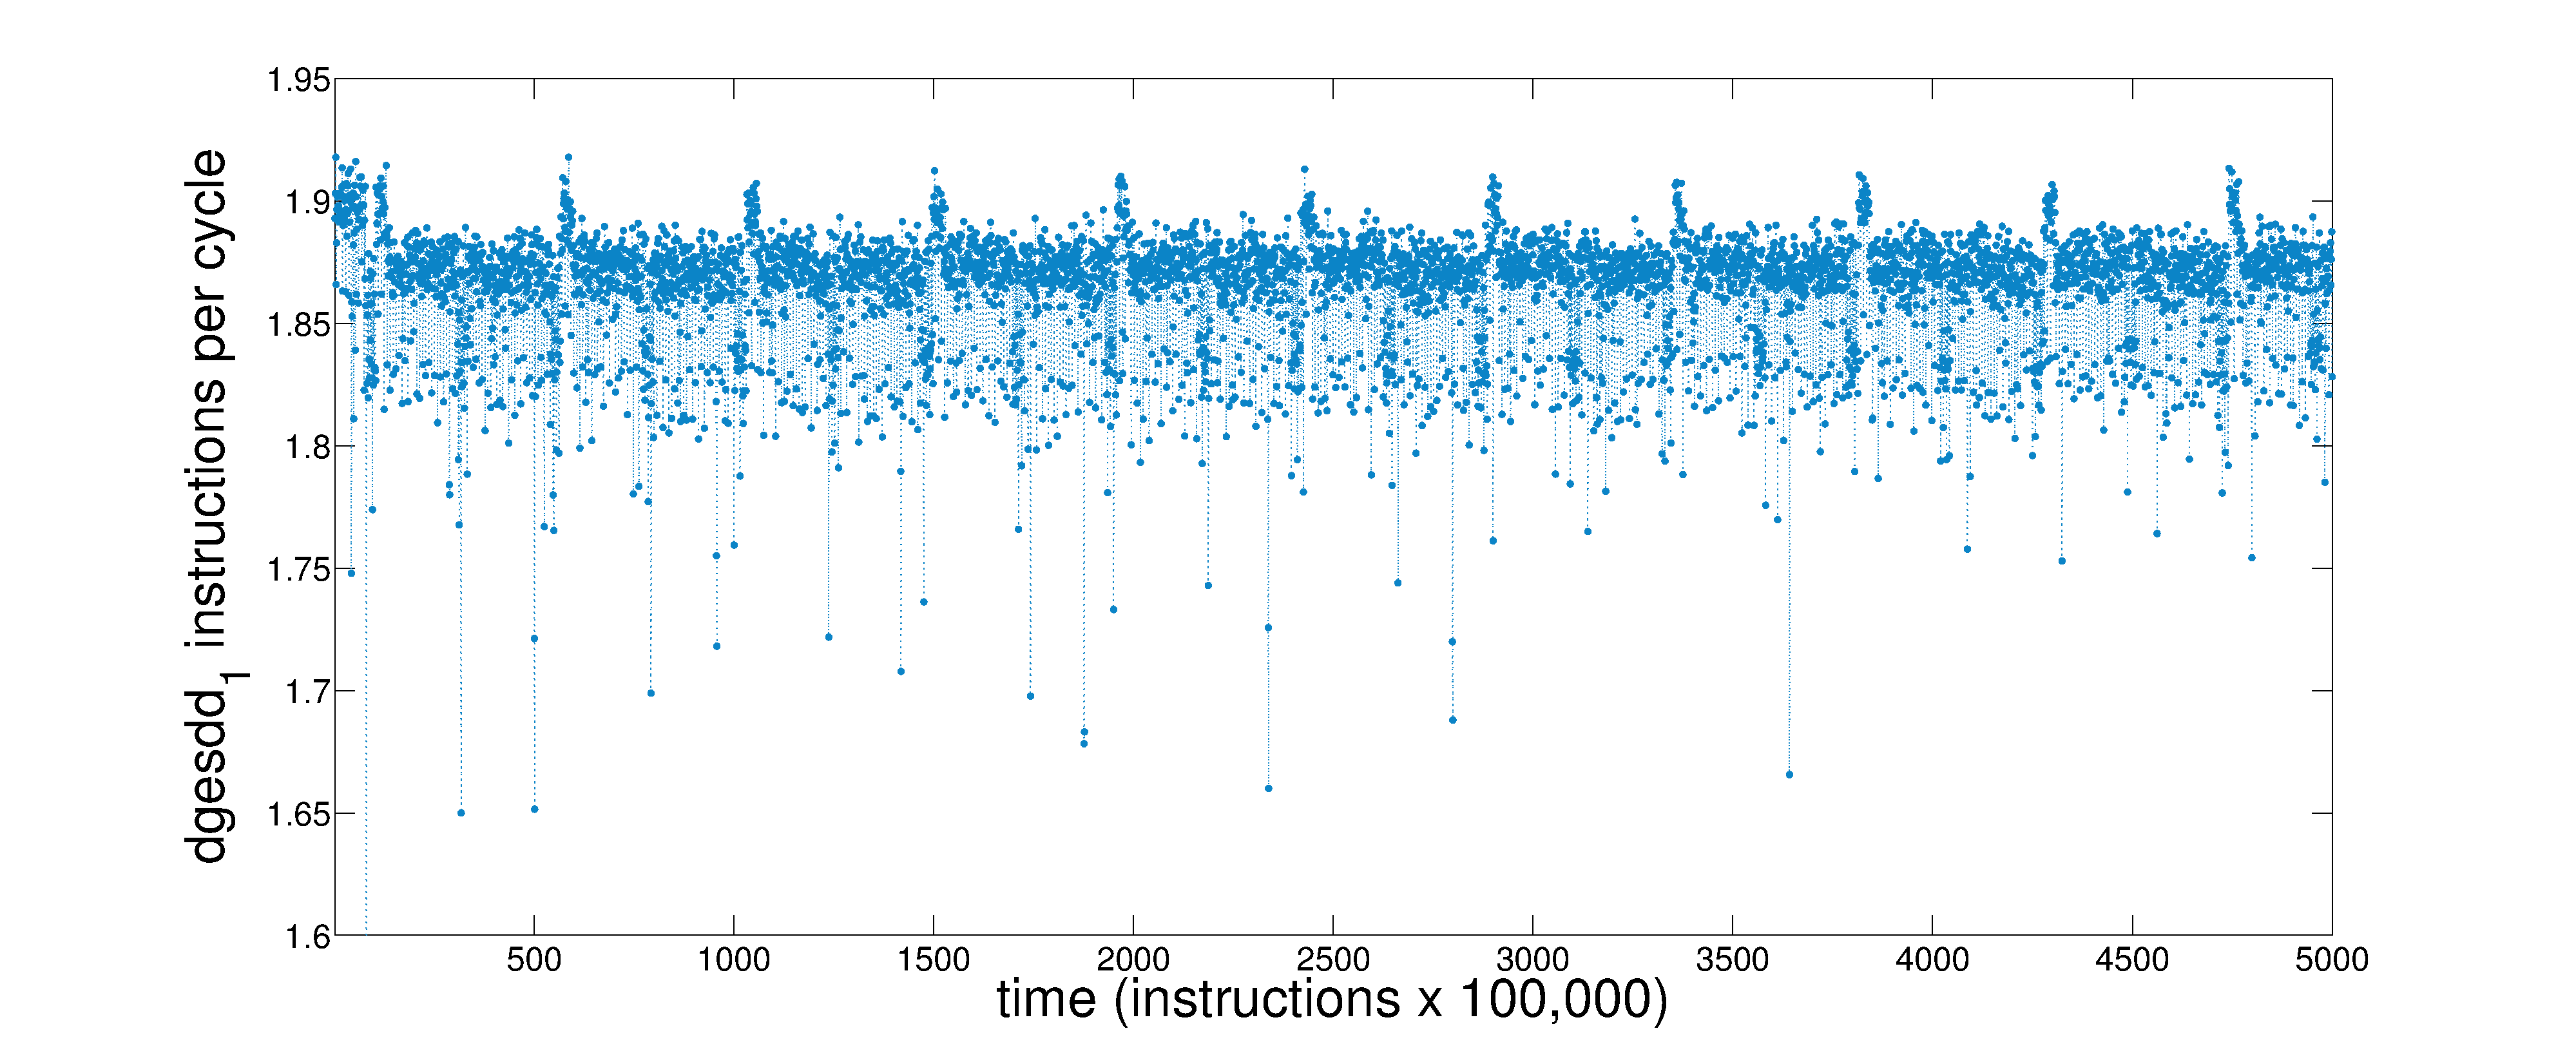
\includegraphics[width=\textwidth]{figs/svdonets2}
\caption{A small portion of the \svdone time series}\label{fig:svdone-ts}
\end{figure} 
is not quite to the level of the worst-case signal described above,
but it poses a serious challenge to random-walk prediction.  It is
dominated by a white-noise regime (between 1.86 and 1.88 on the
vertical scale in the Figure), punctuated by short excursions above
1.9.  In the former regime, which makes up more than 80\% of the
signal, there are frequent dips to 1.82 and occasional larger dips
below 1.8.  These single-point dips are the bane of random walk
forecasting.  In this particular case, roughly 40\% of the forecasted
points are off by the width of the associated dip, which skews the
associated MASE scores.  Signals like this are also problematic for
the naive prediction strategy, since the outliers have significant
pull on the mean, which compounds the effect of the skew in the
scaling factor and creates a large spread in the \svdone MASE values.
For all of these reasons, we view \svdone as an outlier and thus
exclude it from the fit calculation of the dashed line in
Figure~\ref{fig:wpe_vs_mase_best}.

%This portion should justify the following claim%%%%%%%%%%%%%%%%%%%%%%
%\item The way structure/information/complexity is processed internally by a given process plays a crucial role in predictability.
%%%%%%%%%%%%%%%%%%%%%%%%%


Comparing Figures~\ref{fig:lma_pred_vs_ent} and
\ref{fig:arima_pred_vs_ent} also elucidates another key finding:
usable and quantifiable predictive structure can be present in a time
series without a prediction scheme being able to utilize it. In
particular, information may be transferred from past to future through
the present but because of the mechanism the underlying process uses
to process that information (e.g., linear or nonlinear) certain
prediction strategies may be blind to or not be able to efficiently
utilize this information. For example, consider \col, programs like
this have been shown to exhibit deterministic chaos
\cite{mytkowicz09}. If this were the case with \col, an out-of-the-box
linear method like ARIMA would simply be ill-equipped to model and
utilize the kind of structure present, as is evident in Figure
\ref{fig:arima_pred_vs_ent}. In contrast, a nonlinear predictor like
LMA which is built to handle deterministic chaos, can interpret and
utilize this type of structure just fine. We believe that many of the
shifts in forecast accuracy for low-to-moderate WPE programs between
ARIMA and LMA is precisely happening for this reason: Just because
there is forward information transfer, does not mean that an arbitrary
predictor can interpret or utilize it, but luckily WPE can tell us
when this structure is present as shown in Figure
\ref{fig:lma_vs_arima}.

%In Figures~\ref{fig:lma_pred_vs_ent} and \ref{fig:arima_pred_vs_ent} we directly compare the performance of the LMA and ARIMA prediction methods (respectively) to the value of the weighted permutation entropy for all runs of each program under consideration. The LMA MASE values are largely similar to those of the best predictions, primarily because LMA often performed superior to ARIMA (and the na\"ive method). On the other hand, the ARIMA MASE values are largely uncorrelated with WPE values. As was hinted at while discussing the previous results, the fact that ARIMA is uncorrelated with WPE brings about an interesting perspective on information transfer and WPE. The WPE is sensitive to both linear and nonlinear structure. When you have a low WPE and a high ARIMA it could be that the structure WPE is picking up is simply nonlinear structure that LMA can handle but ARIMA cannot. So while ARIMA is consistently out performed by random walk,  there is plenty of structure present as suggested by WPE and taken advantage of by LMA but since it is nonlinear ARIMA can't take it into account and does bad.



%is in large part one of the major findings of this work. More specifically, say we tried to predict an arbitrary noisy real-valued time series with an ``out-of-the-box" prediction strategy like ARIMA as proposed in \cite{autoArima} and say we got inconsistent and bad forecasts, (i.e., perform worse than the na\"ive random walk strategy (MASE$>1$). How do we determine if the prediction strategy is not adequate for the prediction task, or if the signal is simply too complex to predict. If a signal is too complex and too little forward information transfer is present we may not be able to do better than the random walk, in which case we should not worry ourselves over finding a more complicated prediction strategy. However, if we measure the complexity to be low, $\textrm{WPE}<0.85$ (see Fig.~\ref{fig:pred_vs_wpe}) we can most likely do much better than the random walk and should search for more adequate prediction strategies. 


The big picture: Furthermore, since LMA can predict nonlinear behavior
while ARIMA cannot, we see that the clusters in Figure
~\ref{fig:arima_pred_vs_ent} are mostly further to the right than
those in Figure~\ref{fig:lma_pred_vs_ent}.
